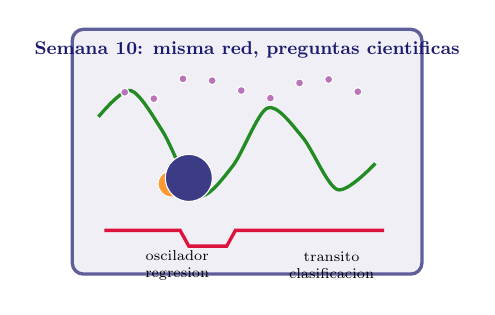
\begin{tikzpicture}[scale=0.74,transform shape]
\draw[fill=MidnightBlue!7,draw=MidnightBlue!70,very thick,rounded corners] (-3.0,-2.1) rectangle (3.0,2.1);
\node[font=\small\bfseries,MidnightBlue] at (0,1.75) {Semana 10: misma red, preguntas cientificas};
\draw[very thick,ForestGreen] plot[smooth] coordinates {(-2.55,0.6)(-2.0,1.05)(-1.45,0.35)(-0.85,-0.75)(-0.25,-0.25)(0.35,0.75)(0.95,0.25)(1.55,-0.65)(2.2,-0.2)};
\draw[very thick,Crimson] (-2.45,-1.35) -- (-1.15,-1.35) -- (-1.0,-1.62) -- (-0.35,-1.62) -- (-0.2,-1.35) -- (2.35,-1.35);
\node[circle,fill=orange!80,draw=white,minimum size=13pt] at (-1.3,-0.55) {};
\node[circle,fill=MidnightBlue!85,draw=white,minimum size=23pt] at (-1.0,-0.45) {};
\foreach \x/\y in {-2.1/1.02,-1.6/0.91,-1.1/1.25,-0.6/1.22,-0.1/1.05,0.4/0.92,0.9/1.18,1.4/1.24,1.9/1.03} {\node[circle,fill=Purple!55,draw=white,inner sep=1.4pt] at (\x,\y) {};}
\node[font=\scriptsize,align=center] at (-1.2,-1.95) {oscilador\\regresion};
\node[font=\scriptsize,align=center] at (1.45,-1.95) {transito\\clasificacion};
\end{tikzpicture}
